\documentclass[a4paper,10pt]{article}
\usepackage[margin=1in]{geometry}
\usepackage{polski}
\usepackage[utf8x]{inputenc}
\usepackage[unicode]{hyperref}
\usepackage{amssymb}
\usepackage{xifthen}
\usepackage[fleqn]{amsmath}
\usepackage{todonotes}
\usepackage{graphicx}
\usepackage{float}
\usepackage{fullpage}
\usepackage{epstopdf}
\usepackage{multirow}
\usepackage{subfig}
\usepackage[europeanresistors,americaninductors]{circuitikz}
\usetikzlibrary{patterns}
\newcommand{\withtodo}{0}


\def\arraystretch{1.2}


\begin{document}

\begin{table}
  \centering
  \def\arraystretch{1.5}
    \begin{tabular}{|l|l|l|l|} \hline
    Wydział:           & \multicolumn{2}{l|}{Dzień:Poniedziałek 14-17}    &Zespół:  \\
    Fizyki             &    \multicolumn{2}{l|}{Data: 20.03.2017}         &8             \\\hline
    Imiona i nazwiska: &Ocena z przygotowania:  &Ocena ze sprawozdania:   &Ocena końcowa: \\
    Marta Pogorzelska  &                        &                         &                \\
    Paulina Marikin    &                        &                         &\\\hline
    \multicolumn{2}{|l|}{Prowadzący:                 } &\multicolumn{2}{l|}{Podpis:             }  \\\hline
  \end{tabular}
\end{table}

\title{Ćwiczenie 43:\\Wyznaczanie $\frac{c_p}{c_v}$ dla powietrza metodą rezonansu akustycznego}
\date{}
\maketitle

\section{Cel badań}
Doświadczenie miało na celu wyznaczenie współczynnika adiabaty dla powietrza.

\section{Wstęp teoretyczny}
$\kappa$ jest współczynnikiem w równaniu adiabaty, zależnym od ilości stopni swobody danego gazu. W modelu gazu doskonałego pomijane są drgania cząsteczek, zaś ich rotacja,
dla cząstek jedno i dwu atomowych, nie wpływa znacząco na interakcje z otoczeniem i także jest pomijana. Definiowany jest on równaniami:

\begin{equation}
  \kappa = \frac{c_p}{c_V} = 1+\frac{1}{n}
\end{equation}
$c_p$ - ciepło własćiwe przy stałym ciśnieniu, $c_V$ - ciepło właściwe przy stałej objętości, n - liczba stopni swobody.
\\\\W tym doświadczeniu jego wartość dla powietrza została wyznaczona metodą Laplace'a, wiążącą równania termodynamiczne z zachowaniem fali akustycznej. Falą taką jest podłużna
fala mechaniczna oscylująca w zakresie częstotliwości słyszalnych dla człowieka. Jej ruch to okresowa kompresja i dekompresja ośrodka zachodząca adiabatycznie, można więc do jego opisania stosować
równanie adiabaty z którego, w połączeniu z równaniem falowym i równaniem Clapeyrona otrzymujemy:

\begin{equation}
  \kappa = \frac{\lambda^2 f^2 M}{kT}
\end{equation}
Dla prędkości fali zmierzonej pośrednio na podstawie równości $v = \lambda f$.
\\\\\\

\section{Opis układu i metody pomiarowej}
Użyte przyrządy:
\begin{itemize}
  \item oscyloskop z podłączonymi sygnałami od generatora i mikrofonu
  \item miarka z podziałką 1mm
  \item głośnik
  \item mikrofon na ruchomym tłoku
  \item rurka z plexi wypełniona powietrzem
  \item regulowany generator sygnału
	\item wzmacniacz sygnału
  \item termometr z podziałką $2^\circ C$
\end{itemize}
Oscyloskop został ustawiony na tryb X-Y, w którym pokazywał krzywą eliptyczną w której x to sygnał z generatora, a y z mikrofonu. W celu wyznaczenia kolejnych długości fali mierzone były
odległości między kolejnymi węzłami, za które uznano maksymalne zwężenie krzywej eliptycznej do prostej. W celu uzyskania kolejnych węzłów manipulowano tłokiem z doczepionym mikrofonem.
Zamiast okresu dla każdej z fal została zmierzona częstotliwość $\omega = 2 \pi T$, mierzona jako odległość między kolejnymi maksimami fali stojącej na
obrazie z oscyloskopu. Temperatura została zmierzona raz, po wykonaniu pozostałych pomiarów.

\section{Pomiary}
\begin{tabular}{lrrrrrrrrr}
okres[$\mu s$] & 250 & 210 & 200 & 180 & 160 & 150 & 140 & 130 & 125 \\\hline
  n   & \multicolumn{9}{l}{odleglość[cm]} \\\hline
  0   & 0.02 & 0.03 & 1.50 & 3.10 & 2.85 & 1.60 & 0.85 & 2.35 & 1.00 \\
  1   & 4.45 & 4.10 & 4.90 & 6.30 & 5.30 & 4.35 & 3.30 & 4.65 & 3.20 \\
  2   & 8.50 & 7.90 & 8.40 & 9.50 & 8.20 & 7.00 & 5.80 & 7.00 & 5.40 \\
  3   &12.70 &11.65 &11.80 &12.60 &11.10 & 9.70 & 8.80 & 9.35 & 7.60 \\
  4   &17.00 &15.55 &15.30 &15.80 &14.00 &12.30 &10.75 &11.70 & 9.70 \\
  5   &21.10 &19.40 &18.65 &19.00 &16.85 &15.00 &13.30 &14.00 &11.90 \\
  6   &25.30 &23.20 &22.10 &22.10 &19.75 &17.30 &15.80 &16.30 &14.10 \\
  7   &29.50 &27.00 &25.70 &25.30 &22.70 &20.30 &18.25 &18.70 &16.25 \\
  8   &33.70 &30.90 &29.00 &28.95 &25.60 &23.00 &20.70 &21.00 &18.40 \\
  9   &37.90 &34.70 &31.75 &31.60 &28.45 &25.70 &23.20 &23.30 &20.50 \\
  10  &42.10 &38.50 &36.00 &34.30 &31.75 &28.30 &25.70 &25.15 &21.80 \\
  11  &46.25 &42.35 &39.50 &37.95 &34.30 &31.00 &28.20 &27.90 &25.00 \\
  12  &&46.20&42.75 &41.10 &37.20 &33.70 &30.70 &30.40 &27.20 \\
  13  &&50.00&46.40 &44.35 &40.10 &36.40 &33.20 &32.65 &29.35 \\
  14  &&&49.90&47.50&42.95 &39.00 &35.65 &34.95 &31.50 \\
  15  &&&&&45.90&41.70&38.15&37.35&33.70 \\
  16  &&&&&48.80&44.45&40.60&39.10&35.80 \\
  17  &&&&&&47.10&43.10&41.90&38.00 \\
  18  &&&&&&49.80&45.60&44.30&40.20 \\
  19  &&&&&&&48.10&46.55&42.40 \\
  20  &&&&&&&&48.90 &44.55 \\
  21  &&&&&&&&&46.70 \\
  22  &&&&&&&&&48.80
\end{tabular}

\section{Analiza pomiarów}

\begin{figure}[H]
  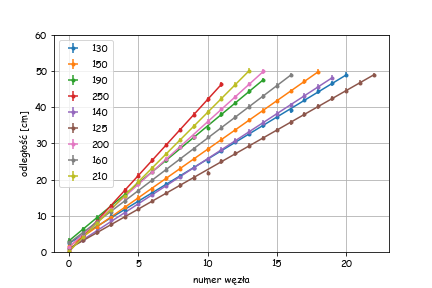
\includegraphics{./Kappa.png}
  \caption{wykres pozwalający wyliczyć długość fali}
  \label{}
\end{figure}
\begin{tabular}{lrrrrrrrrrr}
{} &             k &             M &      T &  $\Delta$T &            f &  $\Delta$f &  $\lambda$ &  $\Delta \lambda$ &  $ \kappa$ &  $\Delta \kappa$ \\
{} & $\frac{J}{K} 10^{-23}$ & Kg $10^{-26}$ & K & K & Hz & Hz & m & m &&\\
0 &  1.3806 &  4.81 &  299.0 &   1.3 &  8000.0000 &   0.0004 &   0.04352 &     0.00014 &   1.4120 &   0.0076 \\
1 &  1.3806 &  4.81 &  299.0 &   1.3 &  7692.3076 &   0.0003 &   0.04638 &     0.00015 &   1.4824 &   0.0081 \\
2 &  1.3806 &  4.81 &  299.0 &   1.3 &  7142.8571 &   0.0003 &   0.0496 &      0.00009 &   1.4644 &   0.0069 \\
3 &  1.3806 &  4.81 &  299.0 &   1.3 &  6666.66667 &   0.00028 &   0.0535 &      0.00008 &   1.4819 &   0.0068 \\
4 &  1.3806 &  4.81 &  299.0 &   1.3 &  6250.00000 &   0.00025 &   0.05785 &     0.00014 &    1.5226 &   0.0076 \\
5 &  1.3806 &  4.81 &  299.0 &   1.3 &  5263.15789 &   0.00017 &   0.06328 &     0.00025 &    1.2922 &   0.0076 \\
6 &  1.3806 &  4.81 &  299.0 &   1.3 &  5000.00000 &   0.00016 &   0.06896 &     0.00028 &    1.3849 &   0.0083 \\
7 &  1.3806 &  4.81 &  299.0 &   1.3 &  4761.90476 &   0.00014 &   0.0765 &      0.00004 &    1.5470 &   0.0067 \\
8 &  1.3806 &  4.81 &  299.0 &   1.3 &  4000.00000 &   0.00010 &   0.08376 &      0.00008 &    1.3076 &   0.0057 \\
\end{tabular}
Ostateczny wynik został wyliczony przy użyciu średniej ważonej gdzie wagą była odwrotność niepewności:
\begin{equation}
  \kappa = \sum_{i=1}^{9} \frac{\frac{\kappa_i}{\Delta \kappa_i}}{\frac{1}{\Delta \kappa_i}}
\end{equation}
\section{Analiza niepewności}
Niepewności temperatury i okresu wyliczono z niepewności aparaturowych i eksperymentatora:\\
\begin{equation}
  \Delta(x) = \sqrt{\frac{x_a^2}{3}+\frac{x_e^2}{3}}
\end{equation}
gdzie $x_a$ - niepewność aparatury, zaś $x_e$ - niepewność eksperymentatora równa połowie niepewności aparatury.\\
Za niepewność długości fali przyjęto pierwiastek z kowariancji dopasowanej prostej zwróconej przez funkcję \emph{polyfit} biblioteki \emph{numpy} w Pythonie.
Niepewności częstotliwości i współczynnika adiabaty zostały wyznaczone przy użyciu metody propagacji niepewności.\\
Częstotliwość:
\begin{equation}
  \Delta f = \frac{\Delta T}{T^2}
\end{equation}
$\kappa$:
\begin{equation}
  \Delta \kappa = \sqrt{(\Delta T \frac{\lambda^2 f^2 M}{kT^2})^2+(\Delta f \frac{2\lambda^2 f M}{kT})^2+(\Delta \lambda \frac{2\lambda f^2 M}{kT})^2}
\end{equation}

\section{Wnioski}
Wszystkie wartości $\kappa$ są zbliżone do przewidywanego wyniku 1.4. Potwierdza to teoretyczne przewidywania dla modelu gazu doskonałego.
\\
Zjawisko rezonansu akustycznego pozwala na dokładne i łatwo wykonane wyznaczanie współczynnika adiabaty.Chociaż finalna niepewność jest relatywnie mała (poniżej 1\% wyniku) głównym czynnikiem ją generującym jest temperatura, której dokładność można łatwo poprawić używając lepszego termometru. Także, nieuwzględniane w opracowaniu zmiany temperatury w trakcie doświadczenia mogły prowadzić do odchyleń wyniku.
Otrzymana na końcu $\kappa$ dla powietrza wynosi:
\\ $\kappa = 1.4311$\\


\end{document}
